\documentclass[nobib]{tufte-handout}

\title{Föreläsning 11: Probabilistiska metoden $\cdot$ 1MA020}

\author[Vilhelm Agdur]{Vilhelm Agdur\thanks{\href{mailto:vilhelm.agdur@math.uu.se}{\nolinkurl{vilhelm.agdur@math.uu.se}}}}

%\date{20 februari 2023}


%\geometry{showframe} % display margins for debugging page layout

\usepackage{graphicx} % allow embedded images
  \setkeys{Gin}{width=\linewidth,totalheight=\textheight,keepaspectratio}
  \graphicspath{{graphics/}} % set of paths to search for images
\usepackage{amsmath}  % extended mathematics
\usepackage{booktabs} % book-quality tables
\usepackage{units}    % non-stacked fractions and better unit spacing
\usepackage{multicol} % multiple column layout facilities
\usepackage{lipsum}   % filler text
\usepackage{fancyvrb} % extended verbatim environments
  \fvset{fontsize=\normalsize}% default font size for fancy-verbatim environments

\usepackage{color,soul} % Highlights for text


\include{mathcommands.extratex}

\begin{document}

\definecolor{darkgreen}{rgb}{0.0627, 0.4588, 0.1451}

\maketitle% this prints the handout title, author, and date

\begin{abstract}
\noindent
I denna föreläsning ger vi fler tillämpningar av probabilistiska metoden på olika problem, praktiska och från andra delar av matematiken. Många men inte alla kommer handla om grafer.
\end{abstract}

\section{\texttt{min-bisection}-problemet}

Antag att vi har en grupp personer på en konferens, och vi vill dela upp dem i två lika stora grupper i olika rum. Vi vill att så många som möjligt som känner varandra skall få vara i samma rum -- ekvivalent vill vi alltså minimera mängden vänskapsband mellan rummen.\sidenote[][]{
  Ett annat sätt att motivera det här problemet är att vi har en graf som är för stor för att lagra i minnet på en enda dator, så vi vill använda två datorer och låta var och en av dem lagra hälften. Så länge vad vi vill räkna ut bara handlar om noder på en av de två datorerna kan vi räkna lokalt -- men om vi vill räkna ut något som involverar kanter mellan de två maskinerna måste de kommunicera med varandra, vilket är långsamt.
  
  För att kunna göra snabba beräkningar vill vi alltså hitta ett sätt att dela upp vår graf så att det inte går så många kanter mellan de två delarna. Det här är ett problem som behöver lösas i praktiken, även om man ofta då har fler än två datorer och behöver hitta en minimal $k$-partition av grafen istället.}

\begin{definition}
  Givet en graf $G = (V, E)$ på $2n$ noder är \texttt{min-bisection} problemet att hitta en minimal bisektion av $G$, alltså att hitta en delmängd $A \in \binom{V}{n}$ som minimerar antalet kanter mellan $A$ och $A^c$. Formellt skriver vi
  $$\min_{A \in \binom{V}{n}} \abs{E(A, A^c)}$$
  där $E(A, A^c)$ alltså är mängden av kanter mellan $A$ och dess komplement $A^c$.
\end{definition}

Hur väl kan vi lösa det här problemet? Ibland är det väldigt svårt -- om vi har fyra personer där alla känner alla, alltså grafen är den fullständiga grafen $K_4$, kommer vi alltid att ha $4$ av $6$ kanter mellan de två delarna.

\begin{figure}
  \centering
  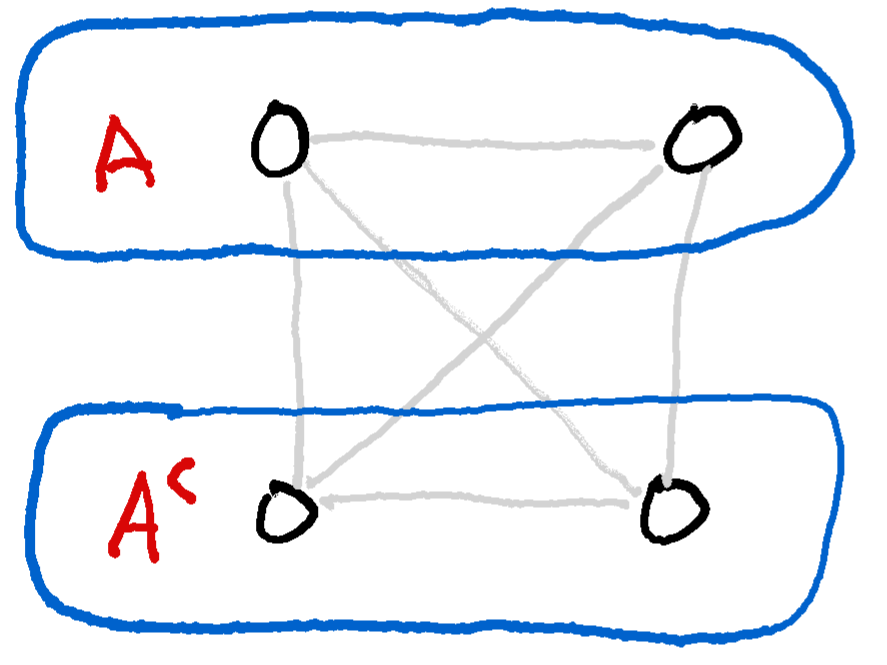
\includegraphics[width=0.5\textwidth]{graphics/K4_min_bisection.png}
  \caption{$K_4$ uppdelad i en bisektion. På grund av symmetrin i grafen är detta så klart enda sättet att dela upp den.}
\end{figure}

Det visar sig att nyckelegenskapen för att kunna göra det här väl är att grafen inte får ha för många kanter relativt antalet noder -- vilket väl inte är allt för överraskande, om man tänker efter.

För att kunna ge en precis variant av det påståendet behöver vi en definition och en sats från grafteorin. Vi utelämnar beviset för satsen, eftersom det inte använder någon sannolikhetsteori.

\begin{definition}
  En Hamiltoncykel i en graf är en cykel som innehåller alla noder exakt en gång. Givet $G = ([n],E)$ kan vi alltså se det som en permutation $\sigma \in S_n$ sådan att $\{\sigma(i),\sigma(i+1)\}$ är en kant för alla $i$, och $\{\sigma(1), \sigma(n)\} \in E$.
\end{definition}

\begin{theorem}[Diracs sats]\sidenote[][]{Inte fysikern, en annan Dirac.}
  Om varje nod i $G = ([n], E)$ har grad\sidenote[][]{Antal grannar.} minst $\frac{n}{2}$ så finns det en Hamiltoncykel i $G$.
\end{theorem}

Vi kan använda denna sats för att bevisa följande resultat:

\begin{proposition}
  Låt $G = ([n], E)$ vara en graf på ett jämnt antal noder, och antag att varje nod har grad högst $\frac{n}{2}$. Då existerar det en delmängd $A \in \binom{[n]}{n/2}$ sådan att
  $$\abs{E(A, A^c)} \leq \frac{\abs{E}}{2}.$$ 

  \begin{proof}
    Låt $G'$ vara komplementgrafen till $G$ -- alltså grafen där det finns en kant mellan varje par av noder som \emph{inte} har en kant mellan sig i $G$, och som inte har en kant mellan par av noder som har en kant i $G$.

    Vi ser enkelt att graden av $i$ i $G'$ är precis $n$ minus graden av $i$ i $G$, så eftersom $d_i \leq n/2$ i $G$ måste $d_i' \geq n/2$ i $G'$. Alltså kan vi tillämpa Diracs sats och hitta en Hamiltoncykel $\sigma$ i komplementgrafen $G'$.

    Vi kan nu använda denna Hamiltoncykel för att para ihop noder i $G$ -- vi matchar $\sigma(1)$ med $\sigma(2)$, $\sigma(3)$ med $\sigma(4)$, och så vidare. Eftersom detta var en Hamiltoncykel i komplementgrafen är vi alltså garanterade att vi aldrig parar ihop två noder som har en kant mellan sig.

    Vi kan nu skapa oss en slumpmässig delmängd $A \in \binom{[n]}{n/2}$ genom att, för varje par, slumpmässigt välja en av de två noderna att ha med i $A$, och låta den andra vara utanför $A$. Denna delmängd kommer ha rätt storlek eftersom vi väljer en nod ur varje par, så vi måste få precis hälften av noderna.

    Låt oss nu räkna ut väntevärdet av $E(A, A^c)$. Vi får att
    \begin{align*}
      \E{E(A, A^c)} &= \E{\sum_{e \in E} \ind{e \in E(A, A^c)}}\\
      &= \sum_{e \in E} \E{\ind{e \in E(A, A^c)}}\\
      &= \sum_{e \in E} \Prob{e \in E(A, A^c)}.
    \end{align*}

    Vad är sannolikheten att en viss fix kant $e = \{u, v\}$ går mellan $A$ och $A^c$? Jo, det händer precis när vi valt att $u \in A$ och $v \in A^c$, eller vice versa. Så vi kan räkna att\sidenote[][]{Vi utnyttjar att de är disjunkta händelser för att gå från $\Prob{(u \in A, v \in A^c) \cup (u \in A^c, v \in A)}$ till summan av de två sannolikheterna.}
    $$\Prob{\{u,v\} \in E(A, A^c)} = \Prob{u \in A, v \in A^c} + \Prob{u \in A^c, v \in A}.$$
    
    Nyckeln nu, och anledningen att vi krånglade med Hamiltoncykeln och matchningen, är att händelserna $u\in A$ och $v\in A^c$ måste vara oberoende. Om $u$ är i $A$ eller inte beror på en myntsingling vi gjorde för $u$ och noden den parades ihop med -- så om vi kallar dess partner för $w$ så är $u \in A$ och $w \in A$ inte oberoende, men för alla $v \neq w$ är $u \in A$ oberoende från $v \in A$.

    Så hur vet vi att vårt par $u, v$ i vår räkning inte råkar ha parats ihop, så att händelserna att de ligger i $A$ inte är oberoende? Jo, vi vet ju att det går en kant mellan $u$ och $v$ -- det är därför vi är intresserade av dem -- men det går ingen kant mellan något par av noder vi parat ihop.

    Alltså kan vi fortsätta vår räkning och få
    \begin{align*}
      \Prob{\{u,v\} \in E(A, A^c)} &= \Prob{u \in A, v \in A^c} + \Prob{u \in A^c, v \in A}\\
      &= \Prob{u \in A}\Prob{v \in A^c} + \Prob{u \in A^c}\Prob{v \in A}\\
      &= \frac{1}{2}\cdot\frac{1}{2} + \frac{1}{2}\cdot\frac{1}{2} = \frac{1}{2}
    \end{align*}
    och alltså har vi att
    \begin{align*}
      \E{E(A,A^c)} &= \sum_{e \in E} \Prob{e \in E(A, A^c)}\\
      &= \sum_{e \in E} \frac{1}{2} = \frac{\abs{E}}{2}.
    \end{align*}

    Enligt vårt sedvanliga argument att väntevärdet omöjligen kan vara mindre än varje specifikt värde måste det alltså finnas ett specifikt $A$ sådant att $E(A, A^c) \leq \E{E(A,A^c)} = \frac{\abs{E}}{2}$ och vi har bevisat satsen.
  \end{proof}
\end{proposition}

\section{ACNSL-olikheten och VLSI}

I nästan varje sak vi gjort som involverat grafer så har vi ritat bilder av grafen på tavlan, och försökt göra dessa bilder så tydliga som möjligt. Vi väljer att rita dem så att kanterna inte korsar varandra om de inte absolut måste.

Detta leder oss till en faktisk matematisk fråga: Givet en graf $G$, hur få korsningar mellan kanter kan vi rita den med?

\begin{definition}
  En graf $G$ som vi kan rita helt utan att några kanter korsar varandra kallas för \emph{planär}. I allmänhet betecknar vi det minimala antalet korsningar av kanter i en ritning av $G$ med $cr(G)$.\sidenote[][]{Från engelskans \emph{crossing number}.}
\end{definition}

Låt oss återigen ge ett lemma som vi inte bevisar.

\begin{lemma}\label{newtons_formula_lemma}
  Det gäller för alla grafer $G = (V, E)$ att
  $$cr(G) \geq \abs{E} - 3\abs{V} + 6.$$

  \begin{proof}
    Utelämnas.\sidenote[][]{Idén i beviset är att använda Eulers formel och sedan resonera om att ta bort kanter som korsar andra kanter:
    \begin{lemma}[Eulers formel]
      Om $G = (V, E)$ är planär är
      $$3\abs{V} - 6 \geq \abs{E}.$$
    \end{lemma}
    
    Hur bevisar man Eulers formel? Den är ett specialfall av Eulerkarakteristiken av en polyeder. För en väldigt lång och intressant diskussion av just hur man bevisar detta, och primärt vad det faktiskt innebär att bevisa något, se Imre Lakatos bok \emph{Proofs and Refutations}, som handlar enbart om just det.
    
    Vill man ha en kortare diskussion av detta kan man se till exempel föreläsningsanteckningarna för kursen i grafteori vid detta universitet -- just ämnet med planära grafer är en av de vackrare delarna av den kursen.}
  \end{proof}
\end{lemma}

Anledningen att vi ger den här olikheten är att vi faktiskt kan enkelt härleda en starkare version av samma olikhet med ett probabilistiskt trick. Såsom mycket annan modern matematik är listan av upptäckare lång -- till skillnad från förr i tiden görs merparten av all matematik i samarbeten numera.

\begin{theorem}[Ajtai-Chvatal-Newborn-Szemerédi-Leighton (ACNSL)]
  För varje graf $G = (V,E)$ gäller det att, om $\abs{E} \geq 4\abs{V}$ så är
  $$cr(G) \geq \frac{\abs{E}^3}{64\abs{V}^2}.$$

  \begin{proof}
    För att förenkla vår notation, låt $n = \abs{V}$ och $e = \abs{E}$. Tag ett godtyckligt $p \in (0,1)$.

    Vad vi vill göra är att studera en slumpmässig delgraf $H$ till $G$, som ges av att varje nod i $G$ är med i $H$ med sannolikhet $p$, och varje kant är med om bägge dess ändpunkter är med i $H$.\sidenote[][]{Detta kallas i allmänhet \emph{nodperkolation} på $G$. Perkolationsteori är ett stort ämne i sannolikhetsteorin, med kopplingar till fysiken -- man brukar tänka sig det som en modell för hur vatten sipprar genom sten. Således namnlikheten till perkolatorkaffe.}

    Vi får av Lemma \ref{newtons_formula_lemma} att
    $$cr(H) \geq \abs{E(H)} - 3\abs{V(H)} + 6.$$
    Eftersom denna likhet gäller för \emph{alla} utfall måste den också gälla om vi tar väntevärdet på bägge sidorna,\sidenote[][]{
      Vi kan formulera detta som ett lemma:
      \begin{lemma}
        Om $X(\omega) \geq Y(\omega)$ för varje $\omega \in \Omega$ så är $\E{X} \geq \E{Y}$.

        \begin{proof}
          Vi räknar att
          \begin{align*}
            \E{X} &= \sum_{\omega \in \Omega} X(\omega)\mu(\omega)\\
            &\geq \sum_{\omega \in \Omega} Y(\omega)\mu(\omega) = \E{Y}.
          \end{align*}
        \end{proof}
      \end{lemma}
    } så från väntevärdets linjäritet får vi alltså att
    \begin{equation}\label{eq:H_expectations_ineq}
      \E{cr(H)} \geq \E{\abs{E(H)}} - 3\E{\abs{V(H)}} + 6.
    \end{equation}

    Så låt oss studera vardera av dessa väntevärden. Så vi räknar att
    \begin{align*}
      \E{\abs{V(H)}} &= \E{\sum_{v \in V(G)} \ind{v \in V(H)}}\\
      &= \sum_{v \in V(G)} \Prob{v \in V(H)} = \abs{V(G)}p = np,
    \end{align*}
    och
    \begin{align*}
      \E{\abs{E(H)}} &= \E{\sum_{\{u,v\} \in E(G)} \ind{\{u,v\} \in E(H)}}\\
      &= \sum_{\{u,v\}\in E(G)} \Prob{\{u,v\} \in E(H)}\\
      &= \sum_{\{u,v\}\in E(G)} \Prob{u \in V(H), v \in V(H)}\\
      &= \sum_{\{u,v\}\in E(G)} \Prob{u \in V(H)}\Prob{v \in V(H)} = \abs{E(G)}p^2 = ep^2.
    \end{align*}

    Hur hanterar vi $\E{cr(H)}$? Jo, vi tar en ritning av $G$ som har precis $cr(G)$ korsningar, och räknar hur många av de korsningarna som är kvar när vi suddat ut alla noder och kanter utanför $H$. Det här ger oss en övre begränsning på $cr(H)$ -- det är ju tänkbart att det finns en bättre ritning av $H$ än att bara rita varje nod och kant på samma sätt som de var ritade i $G$.

    För att korsningen skall vara kvar krävs det så klart att bägge kanterna i korsningen är kvar -- och vi har sett att sannolikheten att en enda kant är kvar är $p^2$, så eftersom kanter är kvar oberoende av varandra\sidenote[][]{Förutom om de utgår från samma nod -- men vi kan aldrig tvingas att rita två kanter som utgår från samma nod så att de korsas. (Detta är ganska uppenbart men inte helt trivialt -- fundera ett ögonblick på varför det är sant.)} är sannolikheten att en korsning blir kvar $p^4$.

    Så enligt samma logik som i de andra fallen får vi att $\E{cr(H)} \leq cr(G)p^4$, så om vi sätter in resultatet av våra räkningar i \eqref{eq:H_expectations_ineq} så får vi att
    $$p^4cr(G) \geq p^2e - 3pn + 6$$
    så om vi nu väljer $p = \frac{4n}{e}$ så får vi alltså
    $$\left(\frac{4n}{e}\right)^4 cr(G) \geq \frac{(4n)^2}{e} - 3\frac{4n^2}{e} + 6 > \frac{(4n)^2}{e} - 3\frac{4n^2}{e}$$
    vilket förenklar till påståendet vi sade vi skulle bevisa.
  \end{proof}
\end{theorem}

Varför är det här ett intressant problem? Att rita grafer med så få korsningar som möjligt är inte bara ett estetiskt problem när man ritar saker på en blackboard, utan också ett praktiskt problem när man skall designa kretskort.

Kretskorten har nämligen många olika komponenter, som vi kan tänka oss som noder, som skall kopplas ihop med varandra. Så länge inte kopplingarna korsar varandra kan man helt enkelt måla dit dem, men om de skall korsa behöver man göra något mer komplicerat. Alltså är det av praktiskt intresse att hitta sätt att rita grafer som minimerar antalet korsningar -- problemet i allmänhet med kretskortsdesign kallas för VLSI (Very Large Scale Integration).

\section{Längsta ökande delföljden i en permutation}

Hittills har vi bara definierat vad vi menar med betingad sannolikhet, inte betingade väntevärden. Tolkningen av dessa är precis vad man hade förväntat sig -- väntevärdet av $X$ betingat på en händelse $A$ är precis det genomsnittliga värdet $X$ tar då $A$ inträffat. Den formella definitionen är som följer:

\begin{definition}
  För varje slumpvariabel $X$ och varje händelse $A$ ges väntevärdet av $X$ betingat på $A$ av
  $$\E{X \given A} = \sum_{y \in X(\Omega)} y \Prob{X = y \given A}.$$
\end{definition}

För en given permutation $\sigma$ av $[n]$ kan vi studera dess ökande och minskande delföljder, såsom vi gjorde i Erd\H{o}s-Székeres sats när vi studerade lådprincipen.

Om vi tar en likformigt slumpmässig permutation, hur lång kommer dess längsta ökande delföljd att vara?

\begin{theorem}
  Om $\sigma_n$ är en likformigt slumpmässig permutation av $[n]$, och $L_n$ är längden hos dess längsta ökande delföljd, gäller det att
  $$\E{L_n} = \Theta\left(\sqrt{n}\right),$$
  det vill säga asymptotiskt är $\E{L_n}$ ungefär $\sqrt{n}$.\sidenote[][]{Formellt är vad vi visar att
  $$\frac{\E{L_n}}{\sqrt{n}} \in [1 - \epsilon(n),e + \epsilon(n)]$$
  för varje $n$, där $\epsilon(n)$ är en funktion som går till noll med $n$, och $e \approx 2.171828$.}

  \begin{proof}
    Låt oss börja med den övre begränsningen av $\E{L_n}$. Att räkna ut ett väntevärde av ett maximum är i allmänhet svårt, så vi behöver någon klokt vald metod för att övre begränsa det här uttrycket.

    Vad vi tänker oss är att vi delar upp i två olika fall -- antingen är den längsta ökande delföljden ``kort'' eller så är den ``lång''. Låt oss säga att den är kort om $L_n \leq \ell$ för något $\ell$ vi väljer senare. Vi har då alltså, genom lagen om total sannolikhet,\sidenote[][]{
      Vi har ju egentligen bara bevisat denna för sannolikheter för händelser, inte för väntevärden av slumpvariabler. Så vi ger det som en övning:
      \begin{xca}
        Bevisa att det, för varje slumpvariabel $X$ och varje händelse $A$, gäller att 
        $$\E{X} = \E{X \given A}\Prob{A} + \E{X \given A^c}\Prob{A^c}.$$
      \end{xca}
    } att
    $$\E{L_n} = \E{L_n \given L_n < \ell}\Prob{L_n < \ell} + \E{L_n \given L_n \geq \ell}\Prob{L_n \geq \ell}.$$

    Nu kan vi hitta olika rimliga övre begränsningar för de två olika termerna. När $L_n$ är ``litet'' kan vi skatta dess längd som $\ell$, och sannolikheten att den blir liten som ett. När $L_n$ är ``stort'' kan vi skatta $L_n$ som $n$, men väljer att vara smartare för att begränsa den lilla sannolikheten $\Prob{L_n \geq \ell}$. Alltså har vi att
    $$\E{L_n} \leq \ell + n \Prob{L_n \geq \ell}.$$

    Låt nu $X_n$ vara antalet ökande delföljder av längd $\ell$, så att vi har att $\Prob{L_n \geq \ell} = \Prob{X_n > 0}$. Enligt samma resonemang med Markovs olikhet som vi använde när vi räknade isolerade noder i en Erd\H{o}s-Rényi-graf har vi att $\Prob{X_n > 0} \leq \E{X_n}$.

    Så om vi, för varje $A = \{a_1, a_2, \ldots, a_\ell\}\in \binom{[n]}{\ell}$, låter $I_A$ vara händelsen att delföljden $\sigma(a_1), \sigma(a_2), \ldots, \sigma(a_\ell)$ är ökande, så har vi alltså att
    $$\E{X_n} = \E{\sum_{A \in \binom{[n]}{\ell}} \ind{I_A}} = \sum_{A \in \binom{[n]}{\ell}} \Prob{I_A}.$$

    Vad är sannolikheten att en viss delföljd är ökande? Jo, det finns totalt $\ell!$ sätt att ordna elementen i delföljden, och bara ett av dem är i ökande ordning. Så sammantaget har vi\sidenote[][]{Här använder vi olikheten $$\ell! \geq e\left(\frac{\ell}{e}\right)^\ell$$ i ett av stegen.} att
    \begin{align*}
      \E{L_n} &\leq \ell + n\Prob{L_n \geq \ell}\\
      &= \ell + n \Prob{X_n > 0} \leq \ell + n \E{X_n}\\
      &= \ell + n \sum_{A \in \binom{[n]}{\ell}} \frac{1}{\ell!} = \ell + n \frac{\binom{n}{\ell}}{\ell!}\\
      &= \ell + \frac{n (n!)}{(n-\ell)!(\ell!)^2} \leq \ell + \frac{n^{\ell + 1}}{(\ell!)^2}\\
      &\leq \ell + n \frac{n^\ell}{\left(e \left(\frac{\ell}{e}\right)^\ell\right)^2}
      \leq \ell + n\left(\frac{e\sqrt{n}}{\ell}\right)^{2\ell}.
    \end{align*}
    Vi kan nu komma ihåg att vi i början av beviset sade att vi skulle välja $\ell$ senare -- och nu ser vi vad vi bör välja $\ell$ som. Specifikt tar vi $\ell = e\sqrt{n} + \epsilon(n)$ för något $\epsilon(n)$ som går till noll med $n$. Då kommer uttrycket inuti exponenten att vara mindre än ett, och således gå till noll, så precis som önskat kommer vi ha att
    $$\E{L_n} \leq e\sqrt{n} + o(1).$$

    För att få vår undre begränsning återanvänder vi en stor del av resonemanget vi hade för att bevisa Erd\H{o}s-Székeres sats. Såsom i den satsen kommer vi vara intresserade både av den längsta ökande och den längsta \emph{minskande} delföljden. Vi observerar att fördelningen för längden av den längsta ökande delföljden och för den längsta minskande delföljden måste vara exakt samma, så vi kan, om vi låter $M_n$ vara längden av den länsta \emph{minskande} delföljden i $\sigma_n$, räkna att
    \begin{align*}
      \E{L_n} &= \frac{\E{L_n} + \E{L_n}}{2}\\
      &= \frac{\E{L_n} + \E{M_n}}{2}\\
      &= \E{\frac{L_n + M_n}{2}} \geq \E{\sqrt{L_n M_n}},
    \end{align*}
    där vi i sista steget använde olikheten mellan det geometriska och aritmetiska medelvärdet.\sidenote[][]{D.v.s. i allmänhet att
    $$\frac{a + b}{2} \geq \sqrt{ab}.$$}

    Så om vi kan bevisa att $L_n M_n \geq n$ för alla permutationer $\sigma$ så är vi klara. Så låt nu, likt i beviset för Erd\H{o}s-Székeres sats, $L_n^k$ vara längden av den längsta ökande delföljden som slutar i $k$, och $M_n^k$ vara längden av den längsta minskande delföljden som slutar i $k$.

    Vad vi observerar är att paren $(L_n^k, D_n^k)$ alla måste vara distinkta från varandra. Ifall vi har $j < k$ måste vi ha antingen $\sigma(j) < \sigma(k)$, och då kan vi förlänga den längsta ökande delföljden som slutar i $j$ genom att lägga till $\sigma(k)$ och sluta i $k$, så att $L_n^j < L_n^k$, eller så har vi $\sigma(j) > \sigma(k)$, och då kan vi genomföra precis samma argument för att få $M_n^j < M_n^k$.

    Alltså måste följden $(L_n^k, D_n^k)$ ha $n$ distinkta element. Dessutom måste alla dessa par så klart ligga i mängden $[L_n] \times [D_n]$ -- så denna mängd måste ha minst $n$ element. Alltså är $L_n D_n \geq n$, och vi är klara.
  \end{proof}
\end{theorem}

\section{Övningar}

\begin{xca}
  Vi introducerade, i en övning till föreläsning 9, konceptet med \emph{turneringar}. En turnering med $n$ lag är ett sätt att rikta $K_n$ -- det är alltså en riktad graf med en kant mellan varje par av noder, där kanten kan peka åt endera hållet. Vi tänker oss det som att alla lag spelar mot alla andra lag, och kanterna pekar från vinnare till förlorare.

  Bevisa att det finns en turnering med $n$ lag som innehåller åtminstone $n!2^{-n}$ Hamiltoncykler.\sidenote[][]{Med Hamiltoncykel i en riktad graf menar vi att vi alltid går i den riktning kanterna pekar -- vi får aldrig lov att gå baklänges längst en kant.}
\end{xca}

%\bibliography{references}
%\bibliographystyle{plainnat}

\end{document}
